% Preambel mit Einstellungen importieren
% Document type and used packages
\documentclass[open=right, % Kapitel darf nur auf rechten Seite beginnen
    paper=A4,               % DIN-A4-Papier
    a4paper,                % DIN-A4-Papier
    12pt,                   % Schriftgöße
    headings=small,         % Kleine Überschriften
    headsepline=true,       % Trennlinie am Kopf der Seite
    footsepline=false,      % Trennlinie am Fuß der Seite
    bibliography=totoc,     % Literaturverzeichnis in das Inhaltsverzeichnis aufnehmen
    twoside=off,             % Doppelseitiger Druck - auf off stellen für einseitig
    DIV=7,
    chapterprefix=true,     % Kapitel x vor dem Kapitelnamen
    cleardoublepage=plain]{scrbook} 

\usepackage{scrpage2}


% Pakete einbinden, die benötigt werden
\usepackage[utf8]{inputenc}       % Dateien in UTF-8 benutzen
\usepackage[T1]{fontenc}          % Zeichenkodierung
\usepackage{graphicx}             % Bilder einbinden
\usepackage[ngerman,english]{babel}       % Deutsch und Englisch unterstützen
\usepackage{xcolor}               % Color support
\usepackage{amsmath}              % Matheamtische Formeln
\usepackage{amsfonts}             % Mathematische Zeichensätze
\usepackage{amssymb}              % Mathematische Symbole
\usepackage{float}                % Fließende Objekte (Tabellen, Grafiken etc.)
\usepackage{booktabs}             % Korrekter Tabellensatz
\usepackage[printonlyused]{acronym}   % Abkürzungsverzeichnis [nur verwendete Abkürzugen]
\usepackage{makeidx}              % Sachregister
\usepackage{listings}             % Source Code listings
\usepackage{listingsutf8}         % Listings in UTF8
\usepackage[hang,font={sf,footnotesize},labelfont={footnotesize,bf}]{caption} % Beschriftungen
\usepackage[scaled]{helvet}       % Schrift Helvetia laden
\usepackage[absolute]{textpos}	  % Absolute Textpositionen (für Deckblatt)
\usepackage{calc}                 % Berechnung von Positionen
\usepackage{blindtext}            % Blindtexte
\usepackage[bottom=40mm,left=35mm,right=35mm,top=30mm]{geometry} % Ränder ändern
\usepackage[square]{natbib}       % Literaturverzeichnis nach DIN mit eckigen Klammern bei \citep
\usepackage{setspace}             % Abstände korrigieren
\usepackage{ifthen}               % Logische Bedingungen mit ifthenelse
\usepackage{scrhack}              % Get rid of tocbasic warnings
\usepackage[pagebackref=false]{hyperref}  % Hyperlinks
\usepackage[all]{hypcap}          % Korrekte Verlinkung von Floats
\usepackage{todonotes}

% Farben definieren
\definecolor{linkblue}{RGB}{0, 0, 100}
\definecolor{linkblack}{RGB}{0, 0, 0}
\definecolor{comment}{RGB}{63, 127, 95}
\definecolor{darkgreen}{RGB}{14, 144, 102}
\definecolor{darkblue}{RGB}{0,0,168}
\definecolor{darkred}{RGB}{128,0,0}
\definecolor{javadoccomment}{RGB}{0,0,240}

% Einstellungen für das Hyperlink-Paket
\hypersetup{
    colorlinks=true,      % Farbige links verwenden       
%    allcolors=linkblue,
    linktoc=all,          % Links im Inhaltsverzeichnis
    linkcolor=linkblack,  % Querverweise
    citecolor=linkblack,  % Literaturangaben
	filecolor=linkblack,  % Dateilinks
	urlcolor	=linkblack    % URLs
}

% Einstellungen für Quelltexte
\lstset{     
      xleftmargin=0.2cm,     
      basicstyle=\footnotesize\ttfamily,
      keywordstyle=\color{darkgreen},
      identifierstyle=\color{darkblue},
      commentstyle=\color{comment}, 
      stringstyle=\color{darkred}, 
      tabsize=2,
      lineskip={2pt},
      columns=flexible,
      inputencoding=utf8,
      captionpos=b,
      breakautoindent=true,
	  breakindent=2em,
	  breaklines=true,
	  prebreak=,
	  postbreak=,
      numbers=none,
      numberstyle=\tiny,
      showspaces=false,      % Keine Leerzeichensymbole
      showtabs=false,        % Keine Tabsymbole
      showstringspaces=false,% Leerzeichen in Strings
      morecomment=[s][\color{javadoccomment}]{/**}{*/},
      literate={Ö}{{\"O}}1 {Ä}{{\"A}}1 {Ü}{{\"U}}1 {ß}{{\ss}}2 {ü}{{\"u}}1 {ä}{{\"a}}1 {ö}{{\"o}}1
}

\urlstyle{same}

% Einstellungen für Überschriften
\renewcommand*{\chapterformat}{%
  \Large\chapapp~\thechapter   % Große Schrift
  \vspace{0.3cm}               % Abstand zum Titel des Kapitels
}

% Abstände für die Überschriften setzen
\renewcommand{\chapterheadstartvskip}{\vspace*{2.6cm}}
\renewcommand{\chapterheadendvskip}{\vspace*{1.5cm}}

\RedeclareSectionCommand[
  beforeskip=-1.8\baselineskip,
  afterskip=0.25\baselineskip]{section}

\RedeclareSectionCommand[
  beforeskip=-1.8\baselineskip,
  afterskip=0.15\baselineskip]{subsection}

\RedeclareSectionCommand[
  beforeskip=-1.8\baselineskip,
  afterskip=0.15\baselineskip]{subsubsection}


% In der Kopfzeile nur die kurze Kapitelbezeichnung (ohne Kapitel davor)
\renewcommand*\chaptermarkformat{\thechapter\autodot\enskip}
\automark[chapter]{chapter}

% Einstellungen für Schriftarten
\setkomafont{pagehead}{\normalfont\sffamily}
\setkomafont{pagenumber}{\normalfont\sffamily}
\setkomafont{paragraph}{\sffamily\bfseries\small}
\setkomafont{subsubsection}{\sffamily\itshape\bfseries\small}
\addtokomafont{footnote}{\footnotesize}
\setkomafont{chapter}{\LARGE\selectfont\bfseries}

% Wichtige Abstände
\setlength{\parskip}{0.2cm}  % 2mm Abstand zwischen zwei Absätzen
\setlength{\parindent}{0mm}  % Absätze nicht einziehen
\clubpenalty = 10000         % Keine "Schusterjungen"
\widowpenalty = 10000        % Keine "Hurenkinder"
\displaywidowpenalty = 10000 % Keine "Hurenkinder"
\renewcommand{\footnotesize}{\fontsize{9}{10}\selectfont} % Größe der Fußnoten
\setlength{\footnotesep}{8pt} % Abstand zwischen den Fußnoten

% Index erzeugen
\makeindex

% Einfacher Font-Wechsel über dieses Makro
\newcommand{\changefont}[3]{
\fontfamily{#1} \fontseries{#2} \fontshape{#3} \selectfont}

% Eigenes Makro für Bilder
\newcommand{\bild}[3]{
\begin{figure}[h]
  \centering
  \includegraphics[width=#2]{#1}
  \caption{#3}
  \label{#1}
\end{figure}}

\newcommand{\source}[1]{\vspace{-3pt} \caption*{ Source: {#1}} }

% Wo liegt Sourcecode?
\newcommand{\srcloc}{src/}

% Wo sind die Bilder?
\graphicspath{{bilder/}}

% Makros für typographisch korrekte Abkürzungen
\newcommand{\zb}[0]{z.\,B.\ }
\newcommand{\dahe}[0]{d.\,h.\ }
\newcommand{\ua}[0]{u.\,a.\ }

% Flags für Veröffentlichung und Sperrvermerk
\newboolean{hsmapublizieren}
\newboolean{hsmasperrvermerk}

% Dokumenteninfos importieren
% -------------------------------------------------------
% Daten für die Arbeit
% Wenn hier alles korrekt eingetragen wurde, wird das Titelblatt
% automatisch generiert. D.h. die Datei titelblatt.tex muss nicht mehr
% angepasst werden.

\newcommand{\hsmasprache}{en} % de oder en für Deutsch oder Englisch

% Titel der Arbeit auf Deutsch
%\newcommand{\hsmatitelde}{Einsatz eines Flux-Kompensators für Zeitreisen mit einer maximalen Höchstgeschwindigkeit von WARP~7}

% Titel der Arbeit auf Englisch
\newcommand{\hsmatitelen}{Performance Comparison between JAVA and Node.js in terms of Scaling in Cloud}

% Weitere Informationen zur Arbeit
\newcommand{\hsmaort}{Mannheim}    % Ort
\newcommand{\hsmaautorvname}{Zheng} % Vorname(n)
\newcommand{\hsmaautornname}{Zeng} % Nachname(n)
\newcommand{\hsmadatum}{11.11.2015} % Datum der Abgabe
\newcommand{\hsmajahr}{2015} % Jahr der Abgabe
\newcommand{\hsmafirma}{Paukenschlag GmbH, Mannheim} % Firma bei der die Arbeit durchgeführt wurde
\newcommand{\hsmabetreuer}{Prof. Peter Knauber, Hochschule Mannheim} % Betreuer an der Hochschule
\newcommand{\hsmazweitkorrektor}{Jens Keller,  SAP SE} % Betreuer im Unternehmen oder Zweitkorrektor
\newcommand{\hsmafakultaet}{I} % I für Informatik
\newcommand{\hsmastudiengang}{IB} % IB IMB UIB IM MTB

% Zustimmung zur Veröffentlichung
\setboolean{hsmapublizieren}{true}   % Einer Veröffentlichung wird zugestimmt
\setboolean{hsmasperrvermerk}{false} % Die Arbeit hat keinen Sperrvermerk

% -------------------------------------------------------
% Abstract

% Kurze (maximal halbseitige) Beschreibung, worum es in der Arbeit geht auf Deutsch
\newcommand{\hsmaabstractde}{}

% Kurze (maximal halbseitige) Beschreibung, worum es in der Arbeit geht auf Englisch

\newcommand{\hsmaabstracten}{}





\begin{document}
\frontmatter

% Römische Ziffern für die "Front-Matter"
\setcounter{page}{0}
\changefont{ptm}{m}{n}  % Times New Roman für den Fließtext
\renewcommand{\rmdefault}{ptm}

% Titelblatt
% -------------------------------------------------------
% In dieser Datei sollten eigentlich keine Veränderungen mehr
% notwendig sein.
% -------------------------------------------------------

\thispagestyle{empty}

% Fakultäten der HS-Mannheim
% -------------------------------------------------------
\ifthenelse{\equal{\hsmafakultaet}{I}}%
  {\newcommand{\hsmafakultaetlangde}{Fakultät für Informatik}%
   \newcommand{\hsmafakultaetlangen}{Department of Computer Science}}{}

\ifthenelse{\equal{\hsmafakultaet}{E}}%
  {\newcommand{\hsmafakultaetlangde}{Fakultät für Elektrotechnik}%
   \newcommand{\hsmafakultaetlangen}{Department of Electrical Engineering}}{}

\ifthenelse{\equal{\hsmafakultaet}{S}}%
  {\newcommand{\hsmafakultaetlangde}{Fakultät für Sozialwesen}%
   \newcommand{\hsmafakultaetlangen}{Department of Social Work}}{}
   
\ifthenelse{\equal{\hsmafakultaet}{B}}%
  {\newcommand{\hsmafakultaetlangde}{Fakultät für Biotechnologie}%
   \newcommand{\hsmafakultaetlangen}{Department of Biotechnology}}{}

\ifthenelse{\equal{\hsmafakultaet}{D}}%
  {\newcommand{\hsmafakultaetlangde}{Fakultät für Gestaltung}%
   \newcommand{\hsmafakultaetlangen}{Department of Design}}{}

\ifthenelse{\equal{\hsmafakultaet}{M}}%
  {\newcommand{\hsmafakultaetlangde}{Fakultät für Maschinenbau}%
   \newcommand{\hsmafakultaetlangen}{Department of Mechanical Engineering}}{}

\ifthenelse{\equal{\hsmafakultaet}{N}}%
  {\newcommand{\hsmafakultaetlangde}{Fakultät für Nachrichtentechnik}%
   \newcommand{\hsmafakultaetlangen}{Department of Information Technology}}{}
   
\ifthenelse{\equal{\hsmafakultaet}{W}}%
  {\newcommand{\hsmafakultaetlangde}{Fakultät für Wirtschaftsingenieurwesen}%
   \newcommand{\hsmafakultaetlangen}{Department of Engineering and Management}}{}
   
\ifthenelse{\equal{\hsmafakultaet}{C}}%
  {\newcommand{\hsmafakultaetlangde}{Fakultät für Verfahrens- und Chemietechnik}%
   \newcommand{\hsmafakultaetlangen}{Department of Chemical Process Engineering}}{}
   

\ifthenelse{\equal{\hsmastudiengang}{IB}}%
  {\newcommand{\hsmastudienganglangde}{Informatik}%
  \newcommand{\hsmastudienganglangen}{Computer Science}%
  \newcommand{\hsmatypde}{Bachelor-Thesis}%
  \newcommand{\hsmatypen}{Bachelor Thesis}%
  \newcommand{\hsmagrad}{\hsmabsc}}{}

\ifthenelse{\equal{\hsmastudiengang}{IMB}}%
  {\newcommand{\hsmastudienganglangde}{Medizinische Informatik}%
  \newcommand{\hsmastudienganglangen}{Medical Informatics}%
  \newcommand{\hsmatypde}{Bachelor-Thesis}%
  \newcommand{\hsmatypen}{Bachelor Thesis}%
  \newcommand{\hsmagrad}{\hsmabsc}}{}
  
\ifthenelse{\equal{\hsmastudiengang}{UIB}}%
  {\newcommand{\hsmastudienganglangde}{Unternehmens- und Wirtschaftsinformatik}%
  \newcommand{\hsmastudienganglangen}{Enterprise Computing}%  
  \newcommand{\hsmatypde}{Bachelor-Thesis}%
  \newcommand{\hsmatypen}{Bachelor Thesis}%
  \newcommand{\hsmagrad}{\hsmabsc}}{}

\ifthenelse{\equal{\hsmastudiengang}{IM}}%
  {\newcommand{\hsmastudienganglangde}{Informatik}%
   \newcommand{\hsmastudienganglangen}{Computer Science}%
   \newcommand{\hsmatypde}{Master-Thesis}%
   \newcommand{\hsmatypen}{Master Thesis}%
   \newcommand{\hsmagrad}{\hsmamaster}}{}

\ifthenelse{\equal{\hsmastudiengang}{MEB}}%
  {\newcommand{\hsmastudienganglangde}{Mechatronik}%
   \newcommand{\hsmastudienganglangen}{Mechatronic}%
   \newcommand{\hsmatypde}{Bachelor-Thesis}%
   \newcommand{\hsmatypen}{Bachelor Thesis}%
   \newcommand{\hsmagrad}{\hsmabsc}}{}
   
\ifthenelse{\equal{\hsmastudiengang}{UB}}%
  {\newcommand{\hsmastudienganglangde}{Automatisierungstechnik}%
   \newcommand{\hsmastudienganglangen}{Automation Technology}%
   \newcommand{\hsmatypde}{Bachelor-Thesis}%
   \newcommand{\hsmatypen}{Bachelor Thesis}%
   \newcommand{\hsmagrad}{\hsmabsc}}{}
   
\ifthenelse{\equal{\hsmastudiengang}{ELB}}%
  {\newcommand{\hsmastudienganglangde}{Elektro- und Informationstechnik/Ingenieurpädagogik}%
   \newcommand{\hsmastudienganglangen}{Elektro- und Informationstechnik/Ingenieurpädagogik}%
   \newcommand{\hsmatypde}{Bachelor-Thesis}%
   \newcommand{\hsmatypen}{Bachelor Thesis}%
   \newcommand{\hsmagrad}{\hsmabsc}}{} 
   
\ifthenelse{\equal{\hsmastudiengang}{EBE}}%
  {\newcommand{\hsmastudienganglangde}{Energietechnik und erneuerbare Energien}%
   \newcommand{\hsmastudienganglangen}{Power Engineering ans Renewable Energies}%
   \newcommand{\hsmatypde}{Bachelor-Thesis}%
   \newcommand{\hsmatypen}{Bachelor Thesis}%
   \newcommand{\hsmagrad}{\hsmabsc}}{}

\ifthenelse{\equal{\hsmastudiengang}{TS}}%
  {\newcommand{\hsmastudienganglangde}{Translation Studies}%
   \newcommand{\hsmastudienganglangen}{Translation Studies}%
   \newcommand{\hsmatypde}{Bachelor-Thesis}%
   \newcommand{\hsmatypen}{Bachelor Thesis}%
   \newcommand{\hsmagrad}{\hsmabsc}}{}
  
\ifthenelse{\equal{\hsmastudiengang}{EM}}%
  {\newcommand{\hsmastudienganglangde}{Automatisierungs- und Energiesysteme}%
   \newcommand{\hsmastudienganglangen}{Automation and Energy Systems}%
   \newcommand{\hsmatypde}{Master-Thesis}%
   \newcommand{\hsmatypen}{Master Thesis}%
   \newcommand{\hsmagrad}{\hsmamaster}}{}
   
\ifthenelse{\equal{\hsmastudiengang}{ELM}}%
  {\newcommand{\hsmastudienganglangde}{Lehramt Ingenieurpädagogik}%
   \newcommand{\hsmastudienganglangen}{Lectureship Educational Engineering}%
   \newcommand{\hsmatypde}{Master-Thesis}%
   \newcommand{\hsmatypen}{Master Thesis}%
   \newcommand{\hsmagrad}{\hsmamaster}}{}
   
\ifthenelse{\equal{\hsmastudiengang}{SAB}}%
  {\newcommand{\hsmastudienganglangde}{Soziale Arbeit}%
   \newcommand{\hsmastudienganglangen}{Social Labour}%
   \newcommand{\hsmatypde}{Bachelor-Thesis}%
   \newcommand{\hsmatypen}{Bachelor Thesis}%
   \newcommand{\hsmagrad}{\hsmaba}}{}
   
\ifthenelse{\equal{\hsmastudiengang}{SAM}}%
  {\newcommand{\hsmastudienganglangde}{Soziale Arbeit}%
   \newcommand{\hsmastudienganglangen}{Social Labour}%
   \newcommand{\hsmatypde}{Master-Thesis}%
   \newcommand{\hsmatypen}{Master Thesis}%
   \newcommand{\hsmagrad}{\hsmamastera}}{}
   
\ifthenelse{\equal{\hsmastudiengang}{BB}}%
  {\newcommand{\hsmastudienganglangde}{Biotechnology}%
   \newcommand{\hsmastudienganglangen}{Biotechnology}%
   \newcommand{\hsmatypde}{Bachelor-Thesis}%
   \newcommand{\hsmatypen}{Bachelor Thesis}%
   \newcommand{\hsmagrad}{\hsmabsc}}{}
   
\ifthenelse{\equal{\hsmastudiengang}{BCB}}%
  {\newcommand{\hsmastudienganglangde}{Biologische Chemie}%
   \newcommand{\hsmastudienganglangen}{Biological Chemics}%
   \newcommand{\hsmatypde}{Bachelor-Thesis}%
   \newcommand{\hsmatypen}{Bachelor Thesis}%
   \newcommand{\hsmagrad}{\hsmabsc}}{}
   
\ifthenelse{\equal{\hsmastudiengang}{BMEBST}}%
  {\newcommand{\hsmastudienganglangde}{Biotechnology - Biomedical Science and Technology}%
   \newcommand{\hsmastudienganglangen}{Biotechnology - Biomedical Science and Technology}%
   \newcommand{\hsmatypde}{Master-Thesis}%
   \newcommand{\hsmatypen}{Master Thesis}%
   \newcommand{\hsmagrad}{\hsmamaster}}{}
   
\ifthenelse{\equal{\hsmastudiengang}{BMEBPD}}%
  {\newcommand{\hsmastudienganglangde}{Biotechnology - Bioprocess Development}%
   \newcommand{\hsmastudienganglangen}{Biotechnology - Bioprocess Development}%
   \newcommand{\hsmatypde}{Master-Thesis}%
   \newcommand{\hsmatypen}{Master Thesis}%
   \newcommand{\hsmagrad}{\hsmamaster}}{}
   
\ifthenelse{\equal{\hsmastudiengang}{BLSM}}%
  {\newcommand{\hsmastudienganglangde}{Life Science Management}%
   \newcommand{\hsmastudienganglangen}{Life Science Management}%
   \newcommand{\hsmatypde}{Master-Thesis}%
   \newcommand{\hsmatypen}{Master Thesis}%
   \newcommand{\hsmagrad}{\hsmamaster}}{}
   
\ifthenelse{\equal{\hsmastudiengang}{KDB}}%
  {\newcommand{\hsmastudienganglangde}{Kommunikationsdesign}%
   \newcommand{\hsmastudienganglangen}{Communication Design}%
   \newcommand{\hsmatypde}{Bachelor-Thesis}%
   \newcommand{\hsmatypen}{Bachelor Thesis}%
   \newcommand{\hsmagrad}{\hsmaba}}{}
   
\ifthenelse{\equal{\hsmastudiengang}{KDM}}%
  {\newcommand{\hsmastudienganglangde}{Kommunikationsdesign}%
   \newcommand{\hsmastudienganglangen}{Communication Design}%
   \newcommand{\hsmatypde}{Master-Thesis}%
   \newcommand{\hsmatypen}{Master Thesis}%
   \newcommand{\hsmagrad}{\hsmamastera}}{}
   
\ifthenelse{\equal{\hsmastudiengang}{MB}}%
  {\newcommand{\hsmastudienganglangde}{Maschinenbau}%
   \newcommand{\hsmastudienganglangen}{Mechanical Engineering}%
   \newcommand{\hsmatypde}{Bachelor-Thesis}%
   \newcommand{\hsmatypen}{Bachelor Thesis}%
   \newcommand{\hsmagrad}{\hsmabsc}}{}
   
\ifthenelse{\equal{\hsmastudiengang}{MM}}%
  {\newcommand{\hsmastudienganglangde}{Maschinenbau}%
   \newcommand{\hsmastudienganglangen}{Mechanical Engineering}%
   \newcommand{\hsmatypde}{Master-Thesis}%
   \newcommand{\hsmatypen}{Master Thesis}%
   \newcommand{\hsmagrad}{\hsmamaster}}{}
   
\ifthenelse{\equal{\hsmastudiengang}{NEB}}%
  {\newcommand{\hsmastudienganglangde}{Elektronik}%
   \newcommand{\hsmastudienganglangen}{Electronics}%
   \newcommand{\hsmatypde}{Bachelor-Thesis}%
   \newcommand{\hsmatypen}{Bachelor Thesis}%
   \newcommand{\hsmagrad}{\hsmabsc}}{}
   
\ifthenelse{\equal{\hsmastudiengang}{TIB}}%
  {\newcommand{\hsmastudienganglangde}{Technische Informatik}%
   \newcommand{\hsmastudienganglangen}{Technical Information Technology}%
   \newcommand{\hsmatypde}{Bachelor-Thesis}%
   \newcommand{\hsmatypen}{Bachelor Thesis}%
   \newcommand{\hsmagrad}{\hsmabsc}}{}
   
\ifthenelse{\equal{\hsmastudiengang}{MTB}}%
  {\newcommand{\hsmastudienganglangde}{Medizintechnik}%
   \newcommand{\hsmastudienganglangen}{Medical Technology}%
   \newcommand{\hsmatypde}{Bachelor-Thesis}%
   \newcommand{\hsmatypen}{Bachelor Thesis}%
   \newcommand{\hsmagrad}{\hsmabsc}}{}
   
\ifthenelse{\equal{\hsmastudiengang}{MTM}}%
  {\newcommand{\hsmastudienganglangde}{Medizintechnik}%
   \newcommand{\hsmastudienganglangen}{Medical Technology}%
   \newcommand{\hsmatypde}{Master-Thesis}%
   \newcommand{\hsmatypen}{Master Thesis}%
   \newcommand{\hsmagrad}{\hsmamaster}}{}
   
\ifthenelse{\equal{\hsmastudiengang}{NM}}%
  {\newcommand{\hsmastudienganglangde}{Informationstechnik}%
   \newcommand{\hsmastudienganglangen}{Informationstechnik}%
   \newcommand{\hsmatypde}{Master-Thesis}%
   \newcommand{\hsmatypen}{Master Thesis}%
   \newcommand{\hsmagrad}{\hsmamaster}}{}
   
\ifthenelse{\equal{\hsmastudiengang}{WB}}%
  {\newcommand{\hsmastudienganglangde}{Wirtschaftsingenieurwesen}%
   \newcommand{\hsmastudienganglangen}{Business Administration and Engineering}%
   \newcommand{\hsmatypde}{Bachelor-Thesis}%
   \newcommand{\hsmatypen}{Bachelor Thesis}%
   \newcommand{\hsmagrad}{\hsmabsc}}{}
   
\ifthenelse{\equal{\hsmastudiengang}{WM}}%
  {\newcommand{\hsmastudienganglangde}{Wirtschaftsingenieurwesen}%
   \newcommand{\hsmastudienganglangen}{Business Administration and Engineering}%
   \newcommand{\hsmatypde}{Master-Thesis}%
   \newcommand{\hsmatypen}{Master Thesis}%
   \newcommand{\hsmagrad}{\hsmamaster}}{}
   
\ifthenelse{\equal{\hsmastudiengang}{VB}}%
  {\newcommand{\hsmastudienganglangde}{Verfahrenstechnik}%
   \newcommand{\hsmastudienganglangen}{Process Engineering}%
   \newcommand{\hsmatypde}{Bachelor-Thesis}%
   \newcommand{\hsmatypen}{Bachelor Thesis}%
   \newcommand{\hsmagrad}{\hsmabsc}}{}
   
\ifthenelse{\equal{\hsmastudiengang}{CB}}%
  {\newcommand{\hsmastudienganglangde}{Chemische Technik}%
   \newcommand{\hsmastudienganglangen}{Chemical Engineering}%
   \newcommand{\hsmatypde}{Bachelor-Thesis}%
   \newcommand{\hsmatypen}{Bachelor Thesis}%
   \newcommand{\hsmagrad}{\hsmabsc}}{}
   
\ifthenelse{\equal{\hsmastudiengang}{CM}}%
  {\newcommand{\hsmastudienganglangde}{Chemieingenieurwesen}%
   \newcommand{\hsmastudienganglangen}{Chemical Engineering}%
   \newcommand{\hsmatypde}{Master-Thesis}%
   \newcommand{\hsmatypen}{Master Thesis}%
   \newcommand{\hsmagrad}{\hsmamaster}}{}

\newcommand{\hsmabsc}{Bachelor of Science (B.Sc.)}
\newcommand{\hsmaba}{Bachelor of Arts (B.A.)}
\newcommand{\hsmamaster}{Master of Science (M.Sc.)}
\newcommand{\hsmamastera}{Master of Arts (M.A.)}
\newcommand{\hsmamasterba}{Master of Business Administration (MBA)}

\newcommand{\hsmakoerperschaftde}{Hochschule Mannheim}
\newcommand{\hsmakoerperschaften}{University of Applied Sciences Mannheim}

\newcommand{\hsmaautorbib}{\hsmaautornname, \hsmaautorvname} % Autor Nachname, Vorname
\newcommand{\hsmaautor}{\hsmaautorvname \ \hsmaautornname} % Autor Vorname Nachname

\ifthenelse{\equal{\hsmasprache}{de}}%
  {\newcommand{\hsmatyp}{\hsmatypde}%
   \newcommand{\hsmathesistype}{zur Erlangung des akademischen Grades \hsmagrad}%
   \newcommand{\hsmakoerperschaft}{\hsmakoerperschaftde}%
   \newcommand{\hsmastudiengangname}{Studiengang \hsmastudienganglangde}%
   \newcommand{\hsmastudienganglang}{\hsmastudienganglangde}%
   \newcommand{\hsmatitel}{\hsmatitelde}%
   \newcommand{\hsmatutor}{Betreuer}%
   \newcommand{\hsmafakultaetlang}{\hsmafakultaetlangde}%
   \selectlanguage{ngerman}}%
  {\newcommand{\hsmatyp}{\hsmatypen}%
   \newcommand{\hsmathesistype}{for the acquisition of the academic degree \hsmagrad}%
   \newcommand{\hsmakoerperschaft}{\hsmakoerperschaften}%
   \newcommand{\hsmastudiengangname}{Course of Studies: \hsmastudienganglang}%
   \newcommand{\hsmastudienganglang}{\hsmastudienganglangen}%
   \newcommand{\hsmatitel}{\hsmatitelen}%
   \newcommand{\hsmatutor}{Tutors}
   \newcommand{\hsmafakultaetlang}{\hsmafakultaetlangen}%
   \selectlanguage{english}}%


% Daten in die Standard-Felder von KOMA-Script eintragen
\titlehead{\hsmatyp\ in\  \hsmastudienganglang}
\subject{}
\title{\hsmatitel}
\author{\hsmaauthor}
\date{\small{\hsmadatum}}

% Daten für das fertige PDF-Dokument
\hypersetup{
  pdftitle={\hsmatitel},  % Titel des Dokuments
  pdfauthor={\hsmaautor},              % Autor
  pdfsubject={\hsmatyp\ in\ \hsmastudienganglang},                % Thema
  pdfkeywords={\hsmatitel}         % Schlüsselworte
}

\newlength{\bindekorrektur}
\newlength{\seitenanfang}
\newlength{\seitenbreite}
  
\setlength{\bindekorrektur}{-46mm}   % Korrektur der horizontalen Position
\setlength{\seitenanfang}{0mm}       % Korrektur der vertikalen Position
\setlength{\seitenbreite}{297mm}

\noindent
\includegraphics[width=7cm]{hsma-logo.pdf}\\

% Titel der Arbeit
\begin{textblock*}{128mm}(45mm,\seitenanfang + 62mm) % 4,5cm vom linken Rand und 6,0cm vom oberen Rand
  \centering\Large\sffamily
  \vspace{4mm} % Kleiner zusätzlicher Abstand oben für bessere Optik
  \textbf{\hsmatitel}
\end{textblock*}%

% Name
\begin{textblock*}{128mm}(45mm,\seitenanfang + 103mm)
  \centering\large\sffamily
  \hsmaautor
\end{textblock*}

% Thesis
\begin{textblock*}{\seitenbreite}(\bindekorrektur,\seitenanfang + 130mm)
  \centering\large\sffamily
  \hsmatyp\\
  \begin{small}\hsmathesistype \end{small}\\
  \vspace{2mm}
  \hsmastudiengangname
\end{textblock*}

% Fakultät
\begin{textblock*}{\seitenbreite}(\bindekorrektur,\seitenanfang + 165mm)
  \centering\large\sffamily
  \hsmafakultaetlang\\
  \vspace{2mm}
  \hsmakoerperschaft
\end{textblock*}

% Datum
\begin{textblock*}{\seitenbreite}(\bindekorrektur,\seitenanfang + 190mm)
  \centering\large 
  \textsf{\hsmadatum}
\end{textblock*}

% Firma
\begin{textblock*}{\seitenbreite}(\bindekorrektur,\seitenanfang + 215mm)
  \centering\large 
  %\textsf{Durchgeführt bei der Firma \hsmafirma}
\end{textblock*}

% Betreuer
\begin{textblock*}{\seitenbreite}(\bindekorrektur,\seitenanfang + 240mm)
  \centering\large\sffamily
  \hsmatutor \\
  \vspace{2mm}
  \hsmabetreuer\\
  \vspace{2mm}
  \hsmazweitkorrektor
\end{textblock*}

% Bibliographische Informationen
\null\newpage
\thispagestyle{empty}
  
\newcommand{\hsmabibde}{\begin{small}\textbf{\hsmaautorbib}: \\ \hsmatitelde \ / \hsmaautor. \ -- \\ \hsmatypde, \hsmaort : \hsmakoerperschaftde, \hsmajahr. \pageref{lastpage} Seiten.\end{small}}

\newcommand{\hsmabiben}{\begin{small}\textbf{\hsmaautorbib}: \\ \hsmatitelen \ / \hsmaautor. \ -- \\ \hsmatypen, \hsmaort : \hsmakoerperschaften, \hsmajahr. \pageref{lastpage} pages. \end{small}}

\ifthenelse{\equal{\hsmasprache}{de}}%
  {\hsmabibde \\ \vspace{0.5cm} \\ \hsmabiben}
  {\hsmabiben \\ \vspace{0.5cm} \\ \hsmabibde}


% Erklärung
\clearpage\setcounter{page}{1}
\thispagestyle{empty}
\textsf{\large\textbf{Erklärung}}

Hiermit erkläre ich, dass ich die vorliegende Arbeit selbstständig verfasst und keine anderen als die angegebenen Quellen und Hilfsmittel benutzt habe.

\ifthenelse{\boolean{hsmapublizieren} \and \not\boolean{hsmasperrvermerk}}%
{
\vspace{0.5cm}
Ich bin damit einverstanden, dass meine Arbeit veröffentlicht wird, d.\,h. dass die Arbeit elektronisch gespeichert, in andere Formate konvertiert, auf den Servern der Hochschule Mannheim öffentlich zugänglich gemacht und über das Internet verbreitet werden darf. 
}{}%


\vspace{1cm}
\hsmaort, \hsmadatum \\

\vspace{1.2cm}						                                      
\hsmaautor

\ifthenelse{\boolean{hsmasperrvermerk}}%
{%
\vspace{11cm}
\color{red}\textsf{\large\textbf{Sperrvermerk}}

Diese Arbeit basiert auf internen und vertraulichen Daten des Unternehmens \hsmafirma.

Diese Arbeit darf Dritten, mit Ausnahme der betreuenden Dozenten und befugten Mitglieder des Prüfungsausschusses, ohne ausdrückliche Zustimmung des Unternehmens und des Verfassers nicht zugänglich gemacht werden.

Eine Vervielfältigung und Veröffentlichung der Arbeit ohne ausdrückliche Genehmigung -- auch in Auszügen -- ist nicht erlaubt.
\color{black}
}{}

\cleardoublepage

% Abstract
\chapter*{Abstract}

\ifthenelse{\equal{\hsmasprache}{de}}%
  {\subsubsection*{\hsmatitelde}\hsmaabstractde\subsubsection*{\hsmatitelen}\hsmaabstracten}
  {\subsubsection*{\hsmatitelen}\hsmaabstracten\subsubsection*{\hsmatitelde}\hsmaabstractde}


% Inhaltsverzeichnis erzeugen
\cleardoublepage
\pdfbookmark{\contentsname}{Contents}
\tableofcontents

% Korrigiert Nummerierung bei mehrseitigem Inhaltsverzeichnis
\cleardoublepage
\newcounter{frontmatterpage}
\setcounter{frontmatterpage}{\value{page}}

% Arabische Zahlen für den Hauptteil
\mainmatter

% Den Hauptteil mit vergrößertem Zeilenabstand setzen
\onehalfspacing

% ------------------------------------------------------------------
% Hauptteil der Arbeit
% Die Arbeit besteht aus Kapiteln (chapter)
\chapter{Introduction}
The promise of cloud has ushered the software engineering into a new era. Technology is to be used anytime and anywhere to untangle issues, provide solutions, bring people together and change their ways of living. This new era of net-centric web-based applications redefines how software is delivered to a customer and how the customer uses the delivered software. The digitization of economy impacts everyone. New businesses and leaders are emerging from nowhere. Companies appear and disappear much faster than ever before. 

SAP, a company which has been renown for its on premise ERP solutions, also faces the pressure from customers to reduce \ac{TCO} and increase agility. It has since long announced its cloud strategy to help customer master the digital economy. The reach of SAP systems is to be extended through cloud based access, ultimately reaching everybody everywhere in entirely new ways. Cloud computing allows on demand software provisioning with Zero-Installation and automatic configuration at low cost and immediate access in ultra-scalable data centers, which leads to the next generation networked solutions. In the process of leverage cloud infrastructure to increase the business agility and to lower the TCO of customers, ultimately new types of applications are enabled.

Cloud solutions come with new capabilities and technical challenges for cloud software development. Different cloud software development platforms and frameworks applied with different programming languages are used inside SAP. Java and Node.JS are the most prominent ones. There have been on-going discussions about how to  take a choice between them for SAP applications considering the SAP environment.\\
Among all the major advantages brought by the cloud paradigm, scalability is the one that makes cloud computing different to an "advanced outsourcing" solution. It’s no secret: high-performance website and web applications drive more traffic, engagement, and increase brand loyalty. In this age where customers are won and lost in a second, continual evaluation and optimization of web properties is essential.  Performance affects customer satisfaction. Slow downs and/or downtime can cost companies thousands of dollars.\\
On account of all the factors named above,  the thesis aims to compare the two server-side technologies: Java and Node.js, in terms of their respective performance and scalibility in a PaaS cloud offering: Cloud Foundry.






 % Externe Datei einbinden\\
\chapter{Related Work}

  \todo[inline]{Write Related Work}
%framework benchmarking
%thesis and published result  % Externe Datei einbindens
% Die Arbeit besteht aus Kapiteln (chapter)
\chapter{Technological Background}
\label{technological background}
Performance and load testing has been conducted ever since applications came into been. There is a sea of different tools available in internet. In the case of this paper, the server's capacity is going to be driven to its limit, after which instead of staying overloaded, the server will try to scale and consume more clients. This requires the testing tool to be capable of generating a large enough amount of end users. 

One of the most popular testing tools is JMeter which is based on Java and cross-platform. It supports multiple protocol and has a very friendly UI to configure test plans. It even produces aggregated test results in different type of graphs. It seems it has everything one asks for except scalibility. When the test requires a bigger scale, JMeter client machine quickly runs into issue that it is unable, performance-wise, to simulate enough users to stress the server or is limited at network level. An option to work around this performance limitation is to utilize remote/distributed testing \index{Cite}\footnote{JMeter Remote Testing \cite{JMeterRemote}}to control multiple remote JMeter engines from a single JMeter client. In this way, one can replicate a test across many low-end computers and thus simulate a larger load on the server. However, remote mode does use more resources than running the same number of non-GUI tests independently. If many server instances are used, the client JMeter can become overloaded, as can the client network connection. Another inconvenience of using JMeter is to find a ideal environment to host it. While one can execute the JMeterEngine on the application server, one can not ignore the fact that this will be adding processing overhead on the application server the testing results will be somewhat tainted. All put together, it is decided not to use JMeter as load generating and testing tool in the project. 

\todo[inline]{Write about CPU & Memory measuring tool}

\todo[inline]{Write about other tools}



  
 % Externe Datei einbindens
\chapter{Experimental Environments}

The experimenting environment is of most importance for technological evaluation. It is also impossible to find a configuration which can do both technologies justice. One can easily end up trapped by some technological limitation of a framework that one used or in the case of this thesis, confined by existing infrastructure provider. However, as the thesis is conducted under the company context, the limitations have to be accepted and taken into account. 

\section{Server in local machine}
Locally a virtual box running in Ubuntu 14.04 with 4 CPUs and 12G memory is installed on host machine which is a Macbook  Pro with 4 CPUs and 16G Memory. However, the application has to share the resource with database and load generator which is not at all a neat configuration. 

\section{Server running environment -  Cloud Foundry}
Cloud Foundry is an open source software bundle that allows you to run a polyglot Cloud Computing \ac{PaaS}. Initially it was developed as a Java \ac{PaaS} for Amazon EC2 by Chris Richardson, in 2009 acquired by SpringSource, which was then acquired by VMWare, then handed over to Pivotal.
The Cloud Foundry Foundation  \citep{Pivotal}  is now the maintainer of Cloud Foundry. More than 50 companies are members of this foundation, such as Pivotal, EMC, HP, IBM, Rackspace, SAP, or VMWare.
The Cloud Foundry PaaS is a multi-component automation platform for application deployment. It provides a scalable runtime environment that can support most frameworks and languages that run on Linux. It also contains many components that simplify deployment and release of microservices applications (for instance, Router, Loggregator, Elastic Runtime (\ac{DEA}), a message bus (NATS), Health Manager, Cloud Controller, etc.)

\subsection{Cloud Foundry at SAP}
Compared with other PaaS offerings, Cloud Foundry has some unique features: it has no limitation on language and framework support and does not restrict deployment to a single cloud.  It is an open source platform that one can deploy to run his apps on his own computing infrastructure, or deploy on an IaaS like \ac{AWS}, vSphere, or OpenStack. In SAP, it is first integrated with SAP Monsoon, then later shifted to Openstack and now hosted in \ac{AWS}. \\
There are two different landscape of Cloud Foundry in SAP. One is called "AWS live". In this landscape, applications run inside containers managed by Warden   \citep{Warden} containerization (a visualization technique providing isolation on operating system level, which is more efficient than virtual machines). The Warden containers including the applications running inside are managed by \ac{DEA} that also monitor the application health and provide the management interface to the Cloud Foundry platform.\\
The other landscape is called "AWS Canary". Instead of \ac{DEA}, each application VM has a Diego Cell   \citep{Diego} that executes application start and stop actions locally, manages the VM’s containers, and reports app status and other data to the \ac{BBS} \citep{BBS} and Loggregator. Instead of Warden, Garden \citep{Garden} is used as the containers to create and manage isolated environments. Diego architecture improves the overall operation and performance, for example supporting Docker containers.

\subsection{ Backing services , Service plans,and Scaling}
Services such as database, authentication form the core of a \ac{PaaS} offering. Cloud Foundry emphasizes on its flexibility in terms of backing services. It distinguishes managed services that obey the Cloud Foundry management APIs, and User-provided Services that serve as adapters to external services. In context of SAP, featured service like Hana database is offered along with other popular SQL and NoSQL databases. These services come with different plans, which define the size and capacity they are capable of offering. For example, PostgreSQL database has a service plan which is delivered in a docker container with predefined maximal number of connections. There are also other plans which provide PostgreSQL in dedicated VMs with different database sizes from extra small to extra large. \\
Service binding in Cloud Foundry is a simple way to tell the application to use a certain backing service. With frameworks like Spring cloud, database connector makes it extremely simple to enable the connection within application. In this thesis, as no extra frameworks is used, application parses the database information from the environment variable \textit{VCAP\_SERVICES} . \\
Since applications and its essential external components are loosely coupled in the context of Cloud Foundry, it leads to easy scalibility which consists the ultimate goals of cloud.  In short, everything is a service: The application, framework functionality (such as persistency), and of course external services to use or integrate with. A service has its own data store, can be implemented and deployed independently, and communicates with other services using lightweight mechanisms.  In this way, horizontal scaling of the system is supported. One can scale services up and down by adding or deleting service instances.

\subsection{Limitations}
As mentioned at the beginning of this chapter, it is impossible to have a perfect environment to conduct a evaluation of the performance of given technology. It is even harder in Cloud Foundry. \\
\subsubsection{Limitation of CPU resource}
\label{cpu limitation}
The first difficulty is to ensure that both applications obtain the equal computing resource. Easiest way is to have JAVA and node applications running on the same VM. However, in Cloud Foundry, applications are not confined to a single cloud. There is no way to secure a dedicated VM on which only the given applications are running. So if one doesn't know if application is running on the same node, one tries to at least make sure both applications have the same CPU allocated. As mentioned above, Cloud Foundry uses containerization which provides operating-system-level visualization instead of simulating bare computing hardware. This means multiple instances running in their respective containers share the same operating system. CPU shares instead of direct CPU time are first distributed. Each container is placed in its own cgroup. Cgroups make each container use a \textit{fair share} of CPU relative to the other containers \citep{CGroup}.This includes two layers of meanings. First, CPU shares are set aside for application according to the memory. Applications with larger amount of memory reservation receive more CPU shares. But does the applications have the same CPU resource when they occupy the same amount of memory? Not necessarily. The second step to designate CPU time is \textit{relative to the other containers}. The following table \ref{CPU time in Cloud Foundry} shows the CPU allocation for 3 applications running in the same VM. 
\begin{table}[h]
	\caption{Example: allocate CPU time in Cloud Foundry}
	\label{CPU time in Cloud Foundry}
	\renewcommand{\arraystretch}{1.2}
	\centering
	\sffamily
	\begin{footnotesize}
		\begin{tabular}{l l l l l }
			\toprule
			\textbf{Application Name} & \textbf{Memory} & \textbf{CPU Shares}& \textbf{CPU Percentage} }& \textbf{State}\\
			\midrule
		    A 	&	100	m & 10 & 20\%   & running\\
			B	&	200 m & 20 & 40\% & running\\
			C	&	200 m &	20 & 40\% & running\\
			\bottomrule
		\end{tabular}
	\end{footnotesize}
	\rmfamily
\end{table}

Nevertheless, this schema of CPU allocation only shows when all the applications are running. If application A now start idling, B and C will both get 50\% of the CPU resources. If only C is running, it gains whole 100\% of the computing power. Now you see why securing identical CPU resource for two applications deployed in Cloud Foundry is impossible. \\
\subsubsection{Limitation of database service}
Cloud Foundry backing services are very convenient to use but is not free of charge when one need a bit more performance. In this thesis, the docker container version of PostgreSQL is used owing to the fact that all other dedicated services cost. The database used in the thesis has a limited connections of 100 per service instance. Luckily,  with connection pooling one application barely needs so many connections. Nevertheless, it does set a threshold on how many instances the application can scale. Large number of scaling is not discussed in the thesis therefore the database is still chosen as default for the performance testing. \\

 \subsubsection{Limitation of proxy server}
 \label{haproxy}
Scalibilty certainly doesn't come for free. The minute system is under stress, the whole landscape of Cloud Foundry is facing challenge. During the thesis, a strange scenario has occurred: the total number of throughput in a minute lingers around 21,000 to 23,000 when the parallel requests reach a certain number. There must be a bottleneck somewhere. Is it because of how the application is implemented? Then the throughput should rise when more application instances are there to handle requests. However, no matter how many application instances are running to relieve the stress, the result stays the same.  The CPU usage of the application doesn't go beyond 20\%. The load is no more than a scratch on the application.\\
Is it because the database simply no longer has enough connection? We can try to give application an additional database. To scale the database is somehow more complicated than scaling the application. Instead of adding one instance to the existing application, another identical application is deployed to Cloud Foundry with its own database instance. The same route is mapped to the new application. Load balancer distributes the requests between two applications. As there are two database instance now, the database capacity is doubled. However, this also changes nothing. To absolutely rule out the limitation is database, the application is pushed to cloud without database at all as a simplest "Hello World" application. The limit of throughput persists. \\ 
Finally, after some searching into existing issues reported from other users, it turns out the bottleneck is in network. Cloud Foundry has a router written in Go, called Gorouter  \citep{Gorouter} which does routing and load balancing. The router performs perfectly and can handle 5,000 requests per second without a hiccup. Nonetheless, Gorouter is not the only thing standing between client and application. The requests coming outside of Cloud Foundry are secured HTTPS calls to keep sensible information from hackers while routes are not encrypted during load balancing. This means before the request is routed to the destination, another server has to terminate SSL and change HTTPS calls to HTTP. This task is accomplished by \ac{HAProxy} \citep{HAProxy} by the time the thesis is finished. HAProxy is never meant to be put in a productive Cloud Foundry landscape owing to its incapability of scaling. Every HAProxy can handle maximum 100 requests per second till its CPU consumption hits the celling. That is when it stops handling any more requests. In the current landscape, there are 4 HAProxy servers. Since they can not scale, it results in a network bottleneck where no more that 400 requests per second can be consumed. This is exactly why the strange scenario come into being. To overcome this restriction, either the proxy server should be changed into scalable ones, which is on the agenda of first quarter 2017 or keeping the connection to Gorouter alive and sending more requests in one decrypted connection. The latter choice is carried out in this thesis which is mentioned in \ref{load generator}.


\section{ Client running environments}
Where the client is running can influence greatly on the performance of the server. Do they share the same database? How great is the network latency? Do they share the same computing resource? To minimize all the influence to zero is next to impossible. Different approaches are discussed in the following. 

\subsection{Client in local machine}
Running server and client in the same physical machine kind of limited the network overhead. However, they consume the same computing resource and inevitably affected by other processes simultaneously operating in the same machine. One client instance won't be enough to generate load to stress application. Regardless, the moment one tries to scale the total of client applications, then it is competing resource with the actual application. This leads to tainted test results.  
\subsection{Client in Cloud Foundry}
Running the client in Cloud Foundry poses less network overhead for the request. Although requests still have to go through HAProxy to arrive at Gorouter despite the fact that client and server are under same domain or even running on the same node. Another convenience to run client on Cloud Foundry is that it is simple to scale. One client instance will have its limitation in sending parallel requests, but one can have as many instances as one needed. This is powerful and essential for this thesis. 

\section{Server and client configuration in the thesis}
\begin{figure}[h]
	\centering
	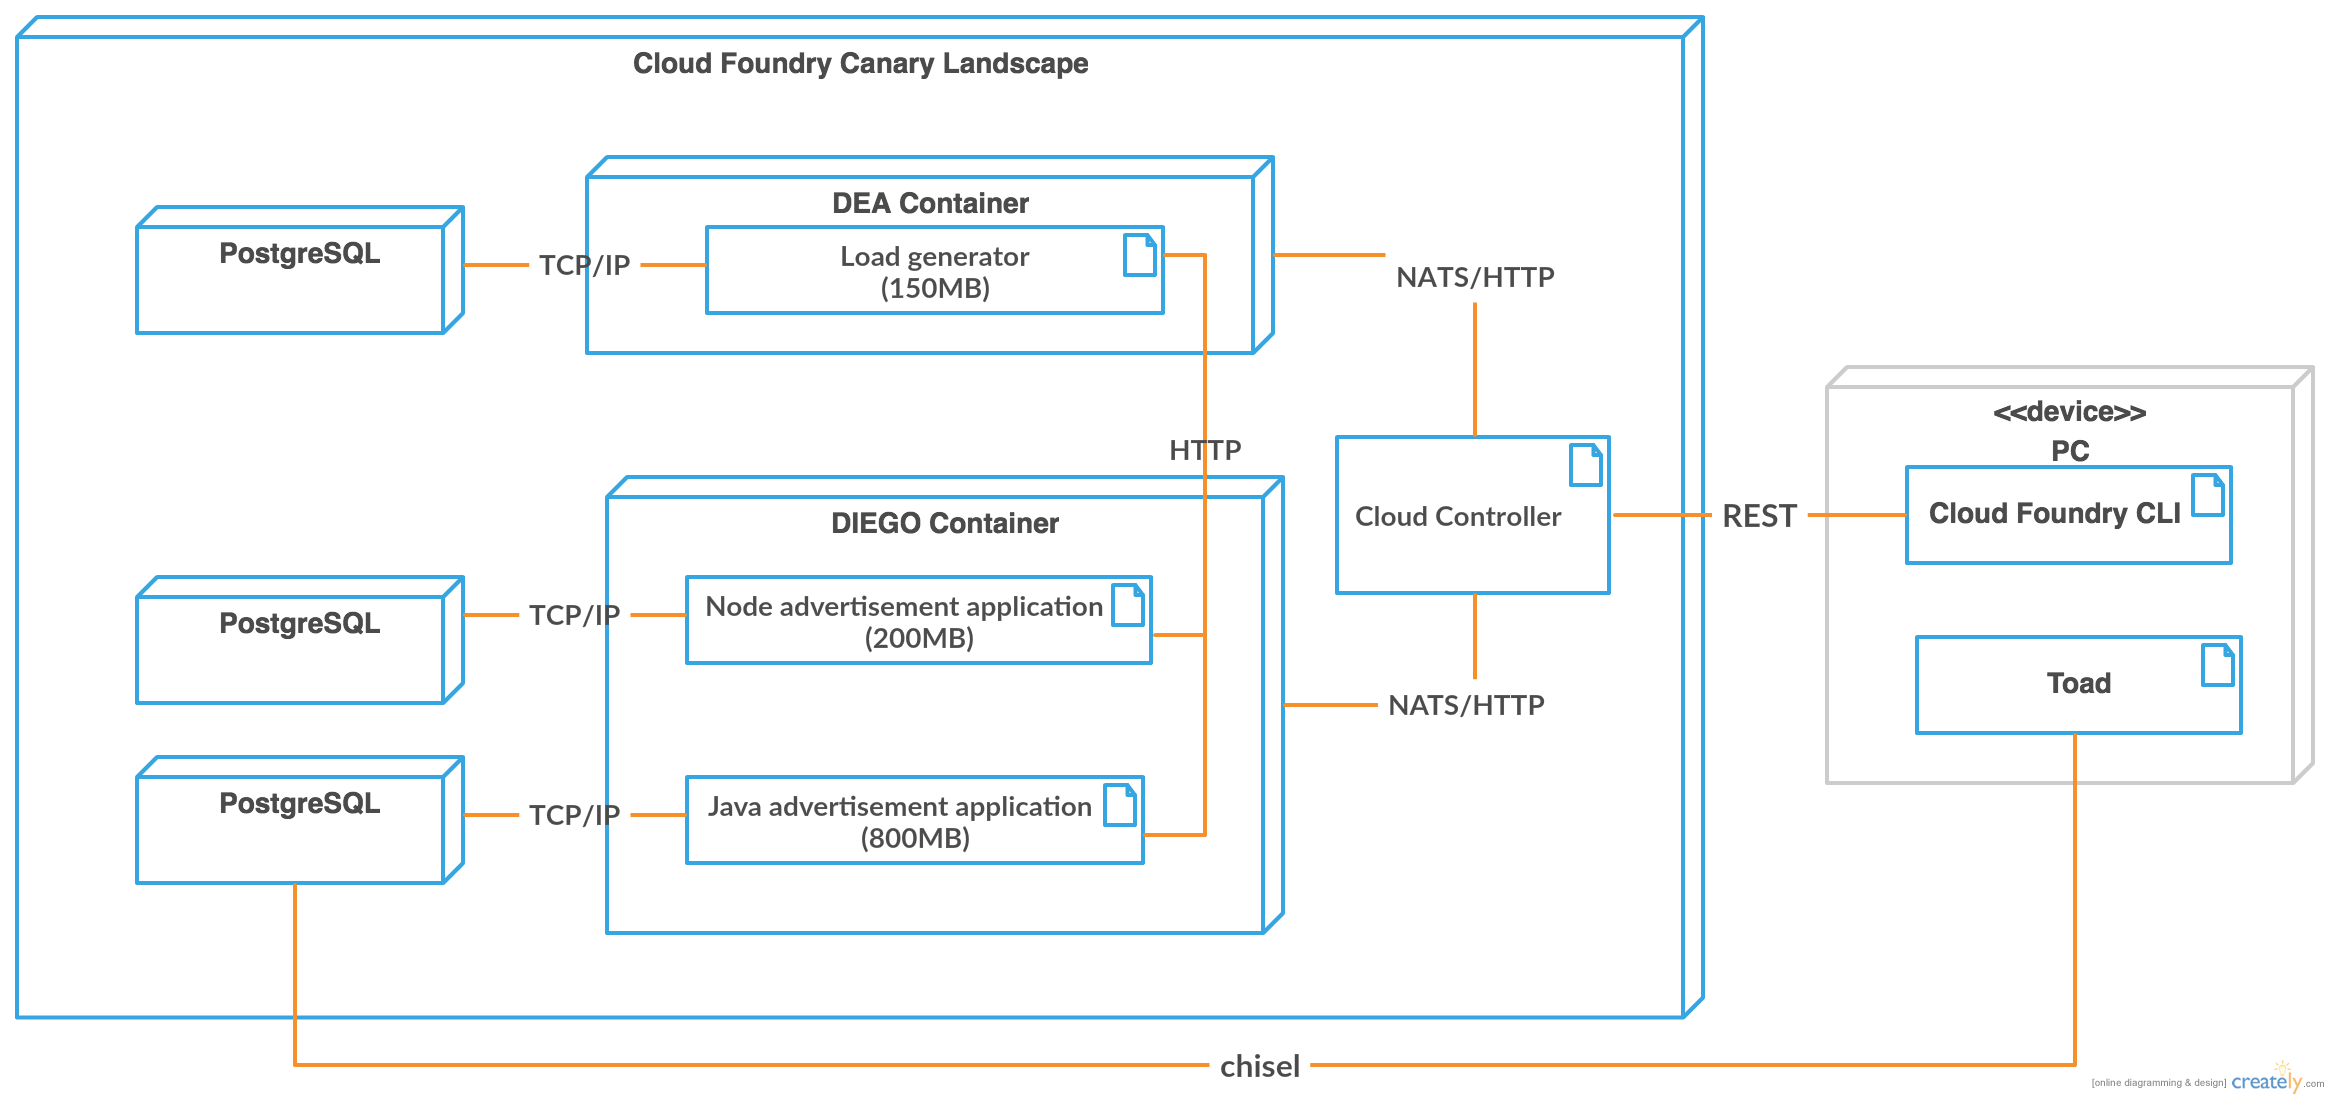
\includegraphics[width=14cm]{deployment_diagram}
	\caption{Deployment diagram for test environment}
	\label{deployment-diagram}
\end{figure}
With all the matters considered, figure \ref{deployment-diagram} shows the final setting of testing environment. First, both client and server are deployed in the same landscape in Cloud Foundry in order to minimize possible network overhead. Second, to avoid the scenario that load generator is running in the same node as the applications, the client and server are deployed into different containers. Clients are in DEA while applications are deployed to Diego. In addition, separate PostgreSQL database services are assigned to applications so that the load on the database is distributed. To retrieve data from database, chisel is used to bring TCP tunnel over HTTP, so that Toad extension on local machine can access the test results. Finally, through Cloud Foundy CLI, requests on application health is made and CPU and memory consumption information is gathered. \\
Another thing to pay attention to is how much memory the applications are allocated. For Java application, 800MB memory is set aside. As mentioned in \ref{memory}, it turns out Java needs about 300MB. However, since Java relies heavily on CPU shares allocated to it, more memory is alloted to ensure it has enough CPU even in a crowded node. On the contrary, Node.js application is given 200MB for the reason that it is single-threaded and more memory doesn't help it gain more computing resource. For the sake of not running into situation of not enough memory due to operational overhead in application such as garbage collector, memory is given quite generously to both applications.  



 % Externe Datei einbinden
\chapter{Testing Tool}
\section{Load generator - a self implemented scalable client}
\subsection{Design and function of load generator}
\subsection{Limitations}
 % Externe Datei einbinden
\chapter{Measuring Tool}
A critical part of performance testing is to ensure as few variables as possible change during each run of the experiment. This generates more consistent results, and allows easier comparison between test runs.\\
In a typical scientific experiment setup, the variables are separated into dependent, independent, and controlled variables. The dependent variables for this testing are of course the throughput and latency numbers that result from performance benchmarking, as well as the CPU and memory usage of the applications during the test runs. For independent variables, the implementation of the application: in Node.js or Java. The exact same tests are running against the two implementations. Besides these variables, everything else is controlled and kept static, for example, applications are deployed to the same cloud landscape to avoid possible falsified  results from different network latencies. \\


\section{Average response time and throughput}
The average response time takes into consideration every round trip.The resulting metric is a reflection of the speed of the web application being tested – the best indicator of how the server is performing from the users’ perspective. The average response time includes the delivery of all resource being used. Thus, the average will be significantly affected by any slow components.\\
In the thesis response time is measured in three different places as you can see from figure \ref{measure-rt}. The first measuring is done by load generator which records the true end-to-end time and throughput. The second checkpoint is the response time retrieved from Logstash which present the round trip from router. Last measuring spot is inside server itself. It reflects the round trip of a query in database. The end-to-end measuring result is used in the final performance analysis while the others serve as tool to determine where is the bottleneck of the performance test is. Since the requests sent from the load generator contains a unique correlation in its header, it is possible to track one request in all the measuring positions. \\

\begin{figure}[h]
	\centering
	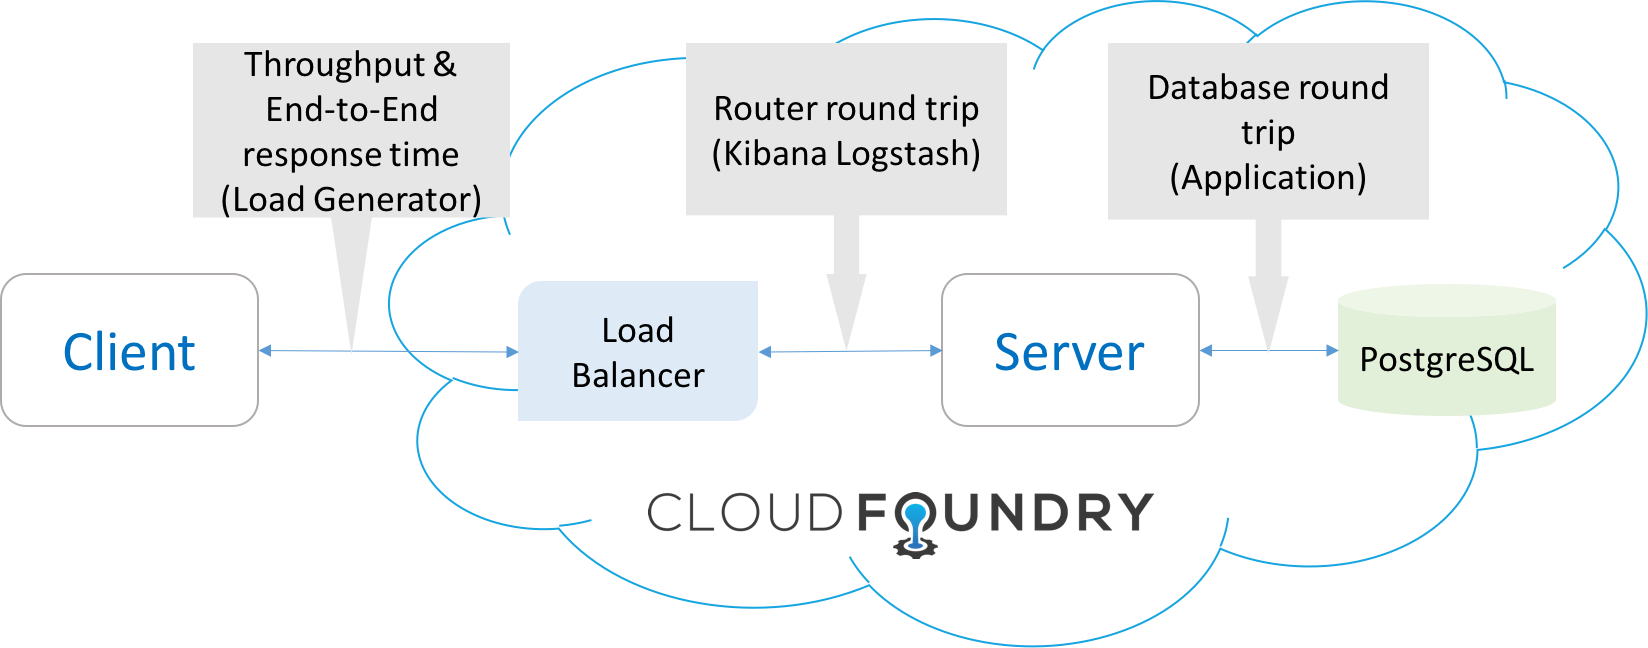
\includegraphics[width=12cm]{measure-rt}
	\caption{Measure response time three different places}
	\label{measure-rt}
\end{figure}

Throughput is the measurement of bandwidth consumed during the test. It shows how much data is flowing back and forth from servers. The requests made to the server in the thesis do not consume data of any significant size, such as images. Therefore the throughput would directly reflect successfully handled amount of requests during the load testing. \\
\subsection{Recording with Load Generator and its limitations}
 In chapter \ref{load generator}, it is discussed how the load generator drives loads. It carries another duty to record the end-to-end response time for each request. Together with response time it also stores the correlation id and start time for each request. The data is first saved in an array and insert into database at the end of load generating. \\
 However, this information is not enough. It would also be great to know the stored result is resulted from which test settings, like how many application instances or how many parallel requests are sent. Therefore these meta information is given to the load generator and saved along with response time. Since the load generator in this thesis is only a worker, it doesn't provide any API to call with given parameters. All the information external from the generator has to be given as start command. However, in Cloud Foundry one application's start command is defined when it is pushed. This means the generator has to be pushed anew to the Cloud Foundry every time the parameter is changed. A small shell script is written to fulfill the task of pushing. \\
 
 It is easy to scale load generator according to what one needs. On the other hand, it also means the generator has to stay stateless, which results in certain amount of manual work. For example, the same test settings may be carried out in several rounds. The result of different rounds should be saved to compare with each other. Making \textit{testround }a automatically incremented data type is what first comes to mind. Yet it can't be defined like that when there are more than one instance of the generator running. This parameter is hence manually given for every new round of test.\\
 
\subsection{Retrieving data from Logstash and its limitations}
Application involves multiple components to accomplish one little task, for example application server, database, router and so on. Performance test can very easily hit limit of one of the components and converting the test of application into test of a router or database. On account of avoiding such cases, finding and ruling out the bottleneck of all the components are carried out. \\
Network is one of the major causes of bottleneck. Is the router capable of taking in so many requests? The best way is to get the response time from router. Although router is not accessible as a component to the developers, \ac{ELK} \citep{ELK} is integrated into Cloud Foundry at SAP. Router response time is logged as default for every request. The logs produced in the application are saved in Logstash\citep{Logstash} and visualized in Kibana \citep{Kibana}. \\ 
However, in order to compare the router response time with end-to-end response time, just reading the results from visualization in Kibana is not enough. To investigate what causes an exceedingly long response time, one has to seek out the precise request and do the comparison. Kibana's visualization is pretty but more convenient would be directly comparing the figures from Logstash. To retrieve the results, a script is written. It sends a json query to the logstash and then parse the query results and sort out the response time logged by router. Following that the statistics are stored into a database.\\
Of course, the result from Logstash can be very large and takes some time. More strangely the logs appeared to be incomplete. Especially when the load is large. Only ten percent of the requests are retrieved from Logstash. After ruling out there is anything wrong with the application that retrieves the result, it is observed that the logs are always retrieved as bundles of 1000 requests which can be clearly seen from visualization in Kibana. After inquiring the colleagues responsible for ELK on Cloud Foundry,  it turns out there is quota for logs. They don't come unlimited. One can only get a certain total of logs preserved per hour or per day.\\
In spite of incomplete information from Logstash, the comparison from the retrieved data shows the router has no performance bottleneck, at least not at the scale this thesis is aiming for. This leads to the realization of the HAProxy limitation discussed in chapter \ref{haproxy}. 

  \subsection{Recording data inside the application and its limitations}
This would be a very simple task if there is no log limit in Logstash: just log the response time recorded in application and retrieve it from Logstash. With the restriction present, the data has to be saved in database. To elevate the performance of saving such large amount of entries, measures have to be taken: using batch in Java and manipulating array to realize a bulk insert in Node.js. In this thesis, the response time and correlation id are saved in an array for all the requests. Another endpoint is defined inside the application to transfer the statistics in array into database.\\
Looking into the response time from database also helps to discover where the bottleneck of database starts. For example, when testing locally, up to a certain number of parallel requests from load generator, the throughput of the application no longer increases while the average response time goes up. Comparing the response time from database, there is an exact analog from peak of end-to-end response time to the peak in the response time from database.The slower requests also require more time to get database connection. \\
Another thing to be taken into consideration is the memory consumption will grow infinitely if one does not transfer recorded data to database. As said above, the information obtained from the application help to identify the efficiency of database. After the determination of limitation, one no longer needs to analyze the data,  consequently forgets to call the endpoint and transfer the data to database. As a result, the array will accumulate, grow into a considerable size and eventually cause out-of-memory. For example, correlation id is saved as 36-letter \textit{string} which consumes 36 * 2 byte memory. Response time is saved as \textit{long} which takes 16 byte. Putting them together, a request needs 88 byte memory to store the response information. If one round of load test generates 100000 requests. it will result in occupying up to 8 MB memory. A Node.js application as a whole only needs maximum 100 MB to run. Therefore a switch should be built inside the application to turn off recording the data or there should be a central operational endpoint to clean up the array before each load testing. 
\section{CPU and Memory consumption}
In chapter \ref{cpu limitation}, it is described how Cloud Foundry allocate its computing resource. In this thesis, tests are conducted on different days and sometimes it is noticed some out of ordinary fluctuations which can be accounted for by a reallocation of computing resource. Nevertheless, CPU and memory consumption are gathered as key metrics since they are directly related to todays cloud pricing mechanism.
\subsection{Cloud Foundry CLI and its limitations}
Since we have no os-level-access to the direct virtual machine in Cloud Foundry, we can not investigate the node. However, the Cloud Foundry command line interface provides simple command \textit{cf app <app-name>} to check the metrics. However, it is extremely tedious and inconvenient to require for the information from command line. Luckily there is a plugin, \textit{cf statistics} \citep{cfstatistics}, which deliver real-time metrics and statistics data. This plugin displays a terminal dashboard showing current app usage metrics/statistics as shown in graph. It can also stream these metrics as JSON formatted output to stdout. It is decided to use the plugin in the thesis. \\
\begin{figure}[h]
	\centering
	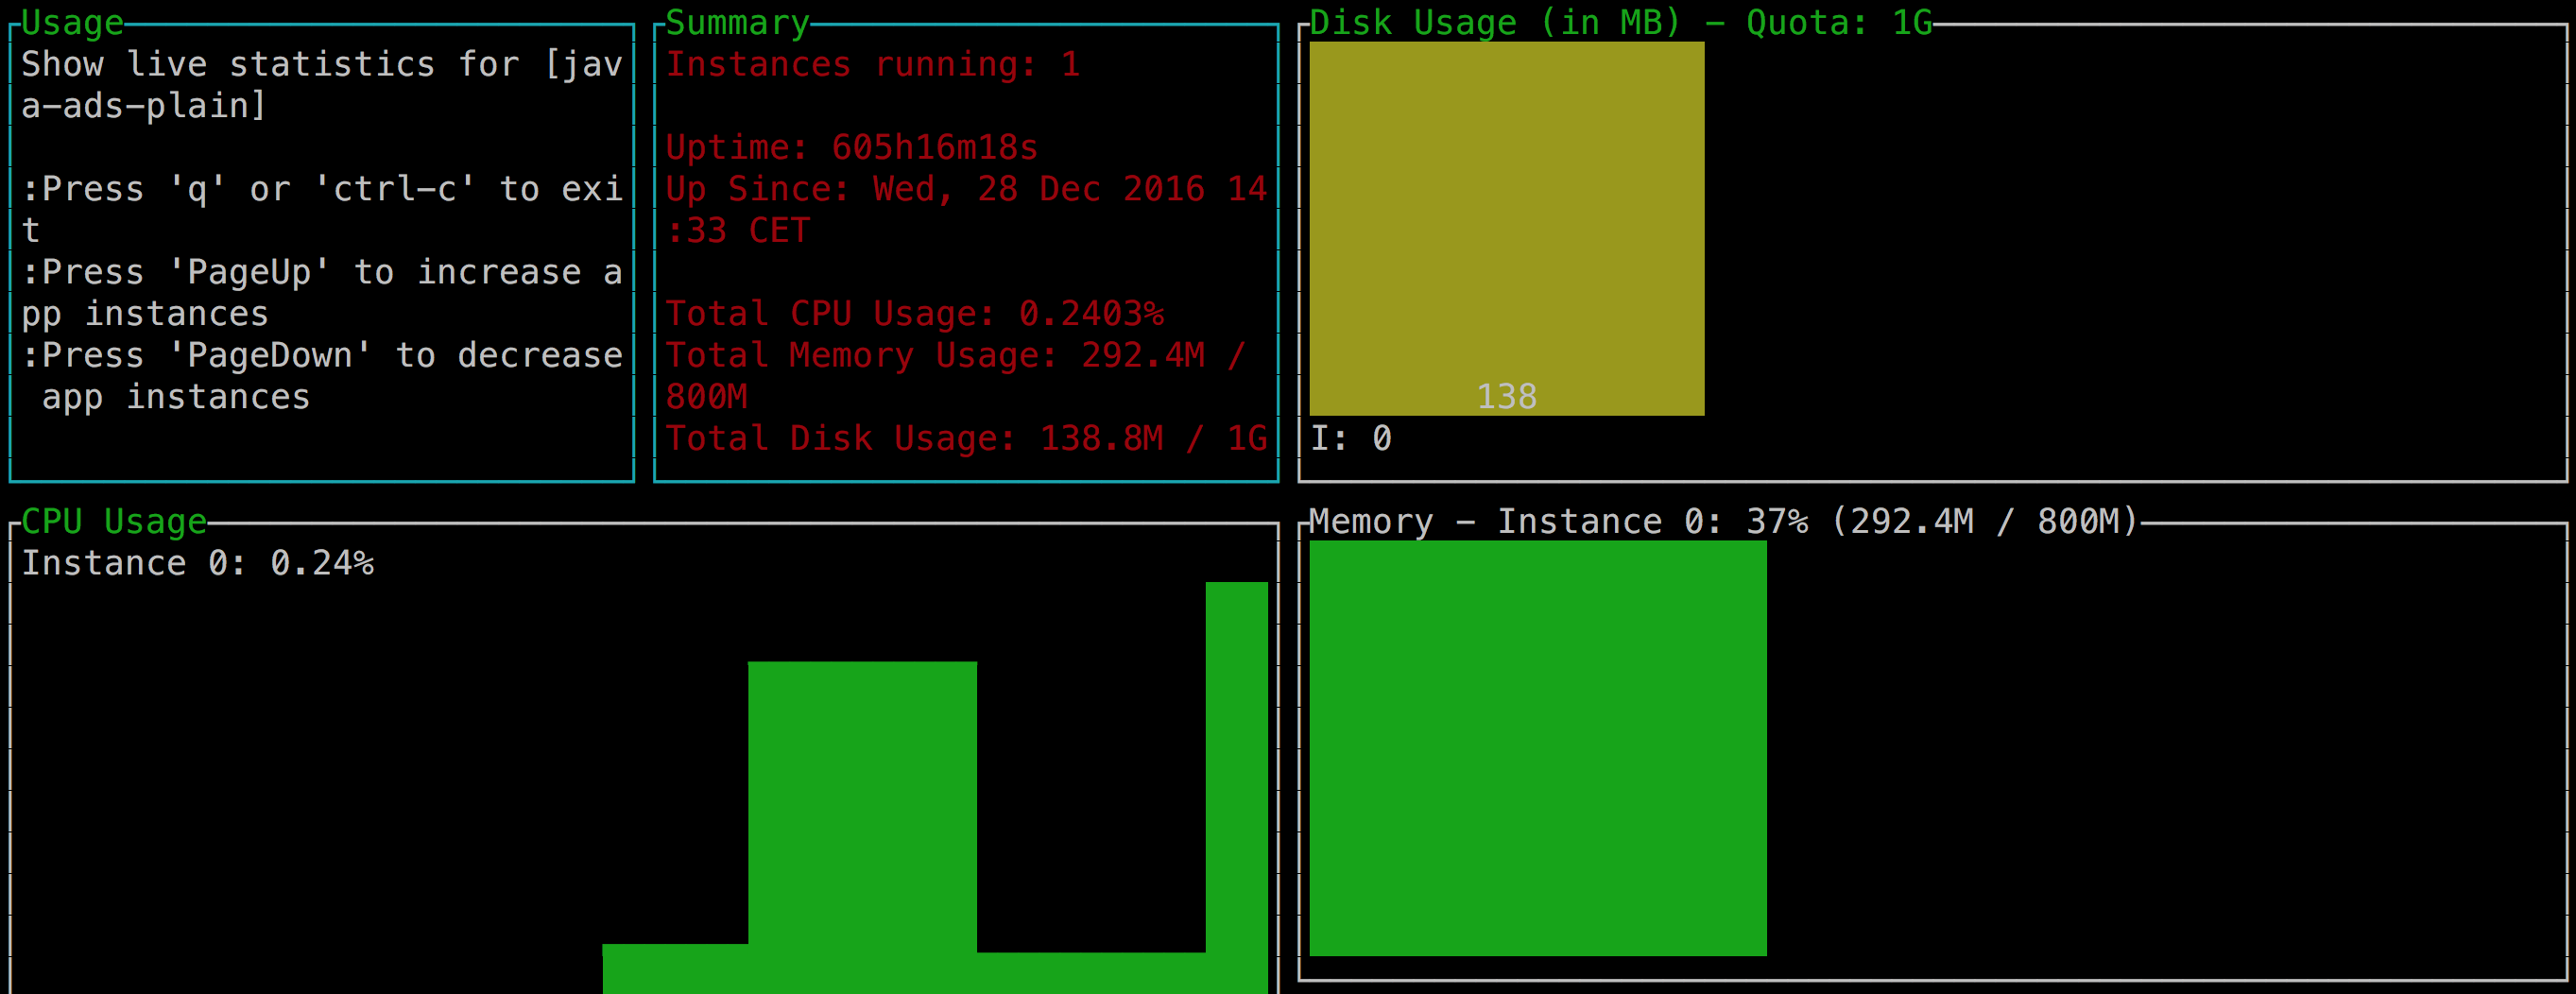
\includegraphics[width=12cm]{cf-statistics}
	\caption{cf statistics display}
	\label{cf-statistics}
\end{figure}
Although this tool is better than the command line, it still requires manual operation. The data gathered can not be stored into database along with other information. After all what the plugin does is only request the API of Cloud Controller  \citep{cloudcontroller} from Cloud Foundry and gather them together. In the long run it would be advised to write one's own application which fetches the information from cloud controller's rest API as part pf the load testing tool. 
\subsection{Memory consumption}
The memory has double meaning in cloud foundry. One can assign a certain amount of max memory to the application which also decides the computing resource an application can get. However, the application doesn't necessarily consume that much. How much memory does an application need to run? It is known, at some point, when the heap reaches its maximum capacity, a full garbage collection will occur, which will bring down the size of the heap memory. Then it will start to grow again and the cycle should continue as long as the application is running. An application with no memory leaks should continue this cycle until the application is stopped. \\
For apps deployed on Cloud Foundry, one way to find out the actual memory to run the application is to let it run under load until the first full garbage collection occurs. The total used memory of the container will continue to grow until this first garbage collection occurs. After that, the memory utilization of the container will stabilize and will not grow any more with sustained load. Figure \ref{memory} shows how the load test is conducted to find out how much memory the application needs to run. 

\begin{figure}[h]
	\centering
	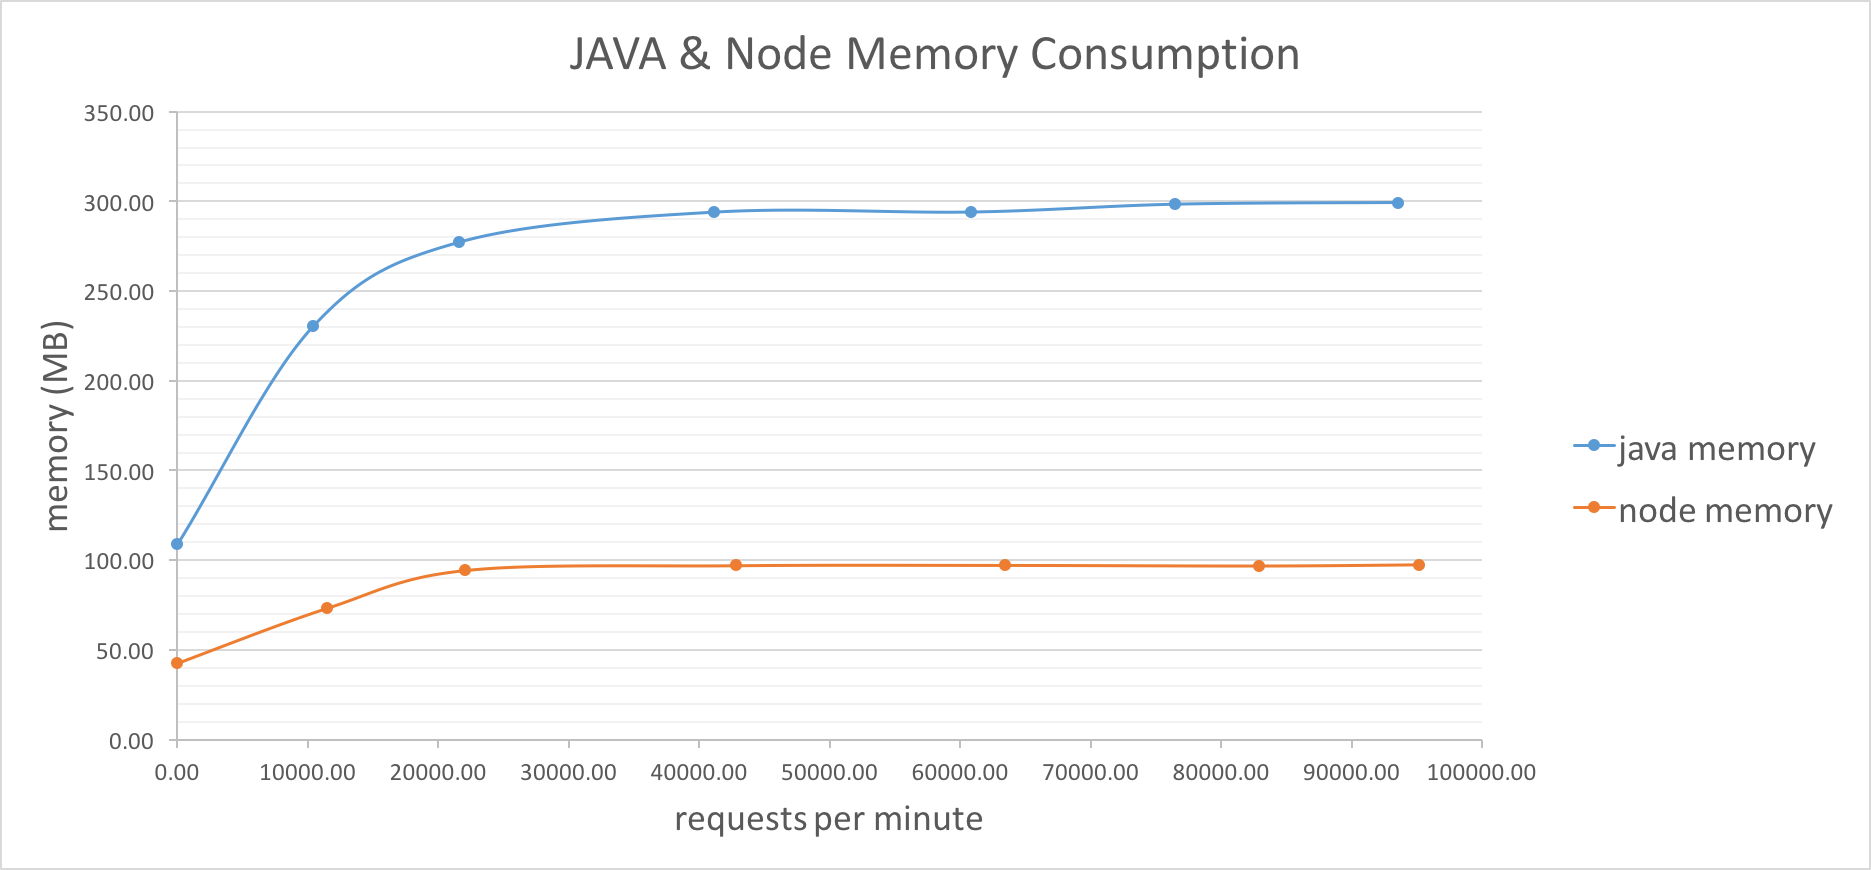
\includegraphics[width=12cm]{memory}
	\caption{Find out the memory Java and Node.js applications need }
	\label{memory}
\end{figure}

\section{Access data from backing service}
In the thesis, raw data instead of aggregated is collected and saved in database in Cloud Foundry.\\
Toad extension for eclipse \citep{toad} is used in the thesis to connect to database and query data. It has no problem connecting to local PostgreSQL, as long as information such as hostname, user, password etc. are provided. Run the command \textit{cf env <application-name>} in Cloud Foundry, one can find a detailed information regarding backing service. For PostgreSQL, exactly the information one needs to establish connection locally are all listed. It seems to be only straightforward to get into the database. However, TCP connection directly to the postgresql back-end service in Cloud Foundry is not possible as the database resides inside the Cloud's subnetwork.\\
Cloud Foundry has provided a solution. It has enabled SSH access to the services in Diego cell \citep{SSH}}. However, if one is behind a cooperate proxy, for example, SAP proxy, the SSH connection cannot be established. \\
Finally, Chisel \citep{chisel} comes to rescue. It is an HTTP client and server which acts as a TCP proxy written in Go. It is an application to be deployed to Cloud Foundry and binded to the target backing service. By starting the application, it maps TCP endpoits of backing services to local workstation and ready to be connected from the toad extension. 

 % Externe Datei einbinden
\chapter{Implementation of Applications}
Store the current order of product and its meta information, find the which shelf stores the current requested product, assign an idling logistic unit to pick up the itinerary ... I/O operations make up the majority of SAP business scenarios. 
 In the load test conducted in this paper, applications are built to realize a scenario: advertisements are published in a bulletin board and clients can browse through the items. 

The PostgreSQL backing service from Cloud Foundry is used as database. As the goal is to test how the application handles large amount of concurrency instead of the database efficiency, data will not be queried in high quantity or complicated joined actions  in the test. 

\section{Implementation Configuration}
To bring Java and node.js to a comparable level, the applications are implemented with minimum use of frameworks so that the overhead or any other influential factors on performance can be first taken off the table.
 \begin{figure}[h]
 	\centering
 	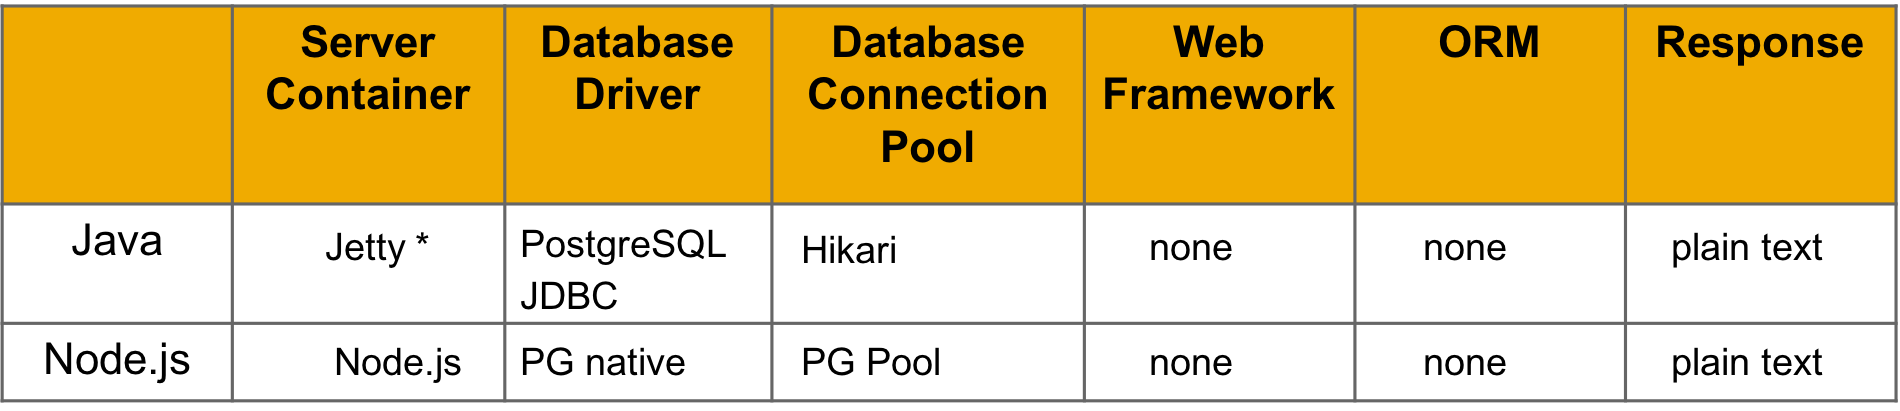
\includegraphics[width=12cm]{implementation}
 	\caption{Implementation configuration}
 	\label{implementation}
 \end{figure}
As table \ref{implementation} shows,  the implementation both applications utilize no REST or any other kind of web framework. No ORM is applied. Response is sent as plain text to the client to avoid overhead brought by JSON serialization. \\
Java application uses embedded Jetty server to handle plain HTTP requests. Node.js application used its embedded web platform. The connection with database is plain JDBC for Java while Node.js uses a popular PostgreSQL library: PG. Since the data structure is intentionally kept simple: only one table and with no complex data types. The application without ORM doesn't bring about a lot of boiler code.  \\

\section{optimize the Java implementation}
All possible attempts are made to bring about every potential performance of the application. Since there is no complex logic, the focus of optimization lays on the interaction between applications and database. In case of Java implementations, to set a optimal thread pool configuration is also investigated. \\
The first checkpoint is database connection which greatly affect performance since it is the most expensive operation in the application without a complicated computing logic. Opening a connection and closing it with every request would gigantically slow down the application. Therefore connection pool is a key component in the implementation. It turns out there are quite a few libraries which handles connection pooling. In the thesis,  three different libraries are tried out. \textit{PGPoolingDataSource}  \citep{pgpool}   comes with default PostgreSQL JDBC driver. \textit{commons-dbcp2} \citep{dbcp} package from Apache Software Foundation provides an opportunity to coordinate the efforts required to create and maintain an efficient, feature-rich package under the \ac{ASF} license. \textit{HikariCP} is a "zero-overhead" production ready connection pool. It turns out \textit{HikariCP} \citep{hikari} has outperformed the other two. \\
The next thing is to find an ideal configuration for the connection pool size. In an article from Brett Wooldridge \citep{hikari}, it is pointed out larger connection pool size configuration doesn't necessarily lead to a better performance. Single core can only execute one thread at a time; then the OS switches contexts and that core executes code for another thread, and so on. It is a basic Law of Computing that given a single CPU resource, executing A and B sequentially will always be faster than executing A and B "simultaneously" through time-slicing. However, there are a few other factors at play. For example, databases typically store data on a disk, which traditionally is comprised of spinning plates of metal with read/write heads mounted on a stepper-motor driven arm. So there is a time cost for disk "I/O wait".  During this time that the OS could put that CPU resource to better use by executing some more code for another thread. So, because threads become blocked on I/O,  more work can be done by having a number of connections/threads that is greater than the number of physical computing cores.
\begin{figure}[h]
	\centering
	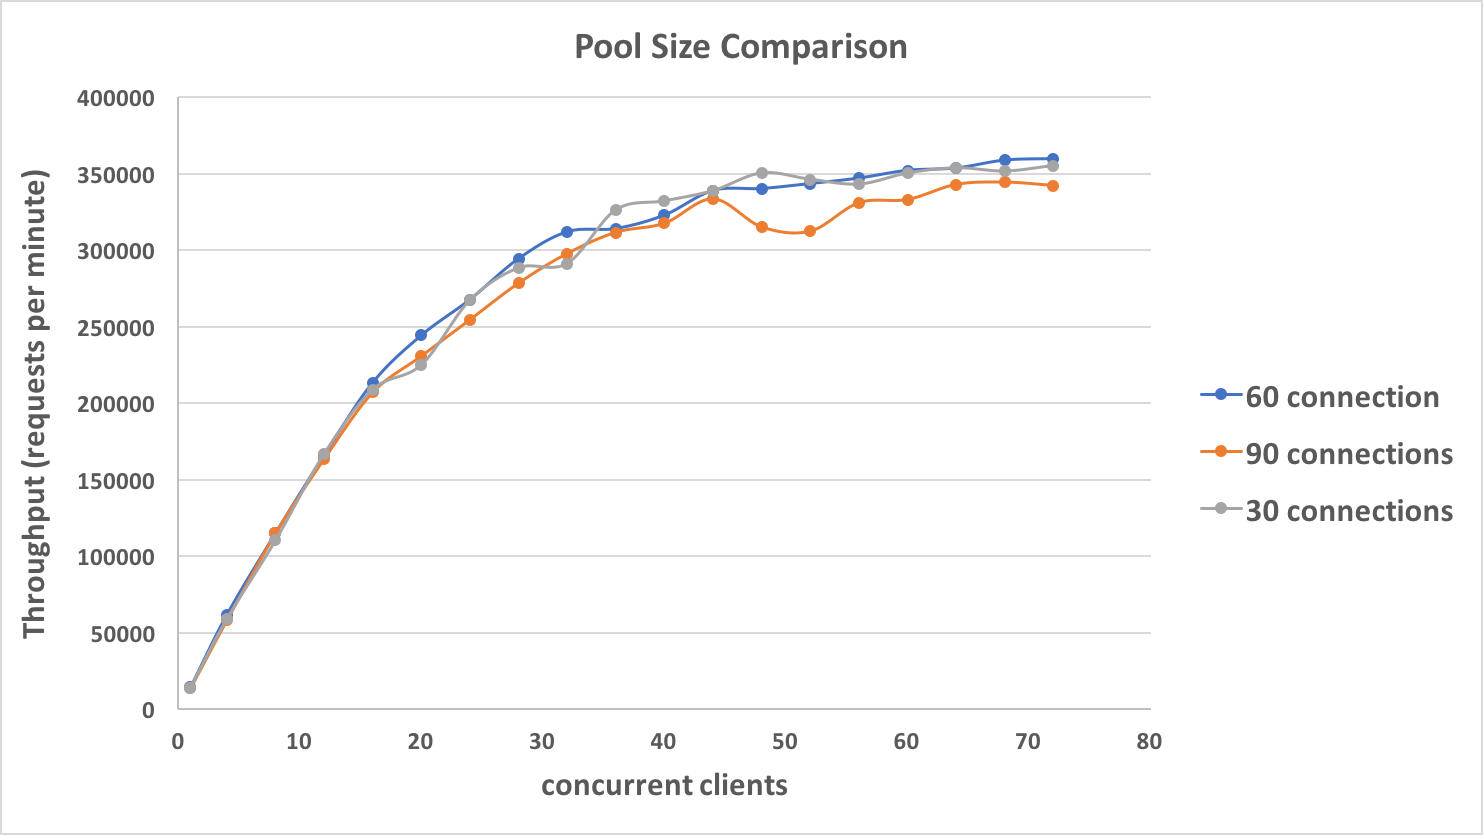
\includegraphics[width=12cm]{pool_size_con_user}
	\caption{Database connection pool size comparison}
	\label{pool-comparison}
\end{figure}
In the case of thesis, database is running in Diego cell which contains 4 CPUs. In order to verify and find the best fit for the load the thesis intend to generate, an experiment is conducted with connection pool size of 30, 60, and 90.  Figure \ref{pool-comparison}, shows a slight difference can be deducted that the pool size of 90 reaches the upper limit of total transaction slightly earlier than the other configurations. A little bit better is the performance from a connection pool size of 60 than that of 30. Then we compared the end-to-end response time with the data base response time.  As figure \ref{ete-vs-db} shows, when the response time peaks, the database response time stays stable and can hardly be considered responsible for the peak. Since the database pool size doesn't pose a conspicuous difference, we can draw the conclusion that the database is working at a high speed with no noticeable delay therefore the pool size setting is not a deciding bottleneck at all. It could be because the database is a docker container version and has no dedicated virtual machine. Thus it lies likely quite near the application and has little network overhead. 

\begin{figure}[h]
	\centering
	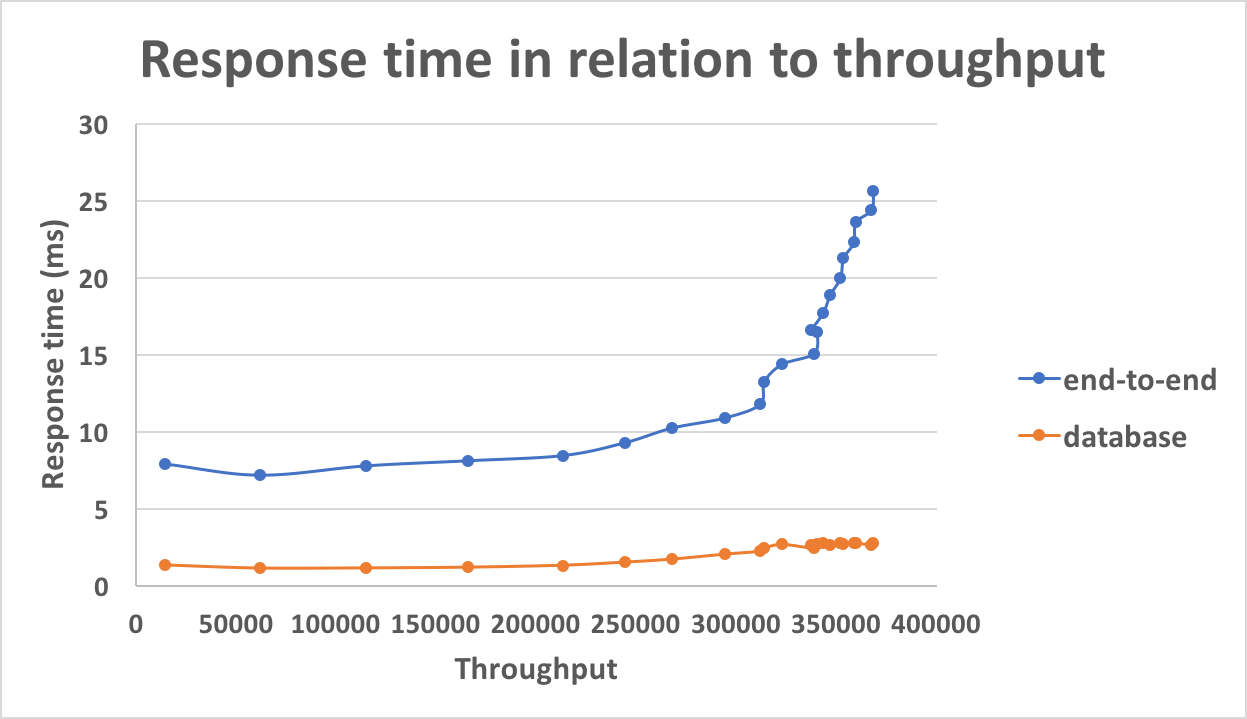
\includegraphics[width=12cm]{ete-vs-db}
	\caption{Comparing end-to-end response time with database response time}
	\label{ete-vs-db}
\end{figure}

Thread pool size is also scrutinized and following the recommendation made by Jetty \citep{threadpool}, the size is set from 10 to 400. \\


\section{optimize the node.js implementation}
Node.js application basically faces the same configuration of connection pool in database. In the thesis, also three different libraries are tried out. Unlike Java libraries, there is some overlapping in regard to the node libraries. In npm, one can find a number of PostgreSQL drivers. However, majority of them are built on the basis of one library: "node-postgres/pg" \citep{node-pg}. They are either wrappers or additional implementation with "promise" or "async/wait". For example, a great difference can not be derived from using of "node-postgres/pg" and "pg-promise" in the scenario in this thesis. The comprehensive research on framework benchmarking \citep{benchmark} uses "Sequelize", which is also tried out in the thesis. However, it yields even a worse performance result because the object mapping costs indisputably computing time. In the end, the suggestion from "node-postgres/pg" writer is adopted to use "pg-native" which can boost a 20-30\% increase in parsing speed.\\




 % Externe Datei einbinden
\chapter{Test Results and Analysis}
\section{IO Intensive}
  \todo[inline]{Write results for local}
  \todo[inline]{Write results for CF}
  \todo[inline]{Write results for monsoon}

\section{Compute Intensive}
  \todo[inline]{Do I need it ?}
 % Externe Datei einbinden
\chapter{Conclusion}
 % Externe Datei einbinden
% ------------------------------------------------------------------

%\label{lastpage}

% Neue Seite
\cleardoublepage

% Backmatter mit normalem Zeilenabstand setzen
\singlespacing

% Römische Ziffern für die "Back-Matter", fortlaufend mit "Front-Matter"
\pagenumbering{roman}
\setcounter{page}{\value{frontmatterpage}}

% Abkürzungsverzeichnis
%\chapter*{Abbreviations}
\addcontentsline{toc}{chapter}{Abbreviations}

\begin{acronym}
\acro{DEA}{Droplet Execution Agents}
\acro{PaaS}{Platform as a Service}
\acro{AWS}{Amazon Web Service}
\acro{IEEE}{Institute of Electrical and Electronics Engineers}
\acro{ISO}{International Organization for Standardization}
\acro{BBS}{Bulletin Board System}
\acro{ELK}{Elasticsearch, Logstash, and Kibana}
\acro{TCO}{Total Cost of Ownership}
\acro{ASF}{Apache Software Foundation}
\end{acronym}


% Tabellenverzeichnis erzeugen
\cleardoublepage
\phantomsection
\addcontentsline{toc}{chapter}{List of Tables}
\listoftables

% Abbildungsverzeichnis erzeugen
\cleardoublepage
\phantomsection
\addcontentsline{toc}{chapter}{List of Figures}
\listoffigures

% Listingverzeichnis erzeugen
\cleardoublepage
\phantomsection
\addcontentsline{toc}{chapter}{Source references}
\lstlistoflistings

% Literaturverzeichnis erzeugen (nach DIN)
%\begin{flushleft}
\bibliographystyle{dinat} % Literatur nach DIN
%\bibliographystyle{abbrv} % Zitate mit [1], [2] etc.
%\bibliographystyle{alpha} % Zitate mit [Kor01], [Vix99] etc.
%\bibliography{literatur}   % BibTeX-Datei mit Literaturquellen einbinden
\end{flushleft}

% Index ausgeben
\cleardoublepage
\phantomsection
\addcontentsline{toc}{chapter}{Index}
\printindex

\end{document}